\graphicspath{{sec03/images/}{sec03/code/s2/}}
\lstset{inputpath=sec03/code/s2/}

\begin{frame}[fragile]{Main idea}\relax
 \centering \Huge {\csk Boxes} and {\csk Glue}
     
\end{frame}

\begin{frame}{Main idea}\relax
\centering \large
\tabcolsep=0.15em
\begin{tabular}{r>{\csk}l}
     A symbol is a & box\\
     it is part of a word, that is a & box\\ 
     the words are connected with & glue\\ 
     into sentances and paragraphs.&\\ 
     A paragraph is a & box\\
     it connected with another one with & glue\\
     to the page. Which is a & box\\
     &\\ 
     by the way: table, picture, ... is a & box 
\end{tabular}

\skfootnote{\wikiC{https://en.wikibooks.org/wiki/LaTeX/Boxes} \knuthc{11}[73]}
\end{frame}

\begin{frame}{Box params}
     
\centering
\newbox\boxtodimen%
\newdimen\hb%
\newdimen\db%
\newdimen\wb%

\setbox\boxtodimen=\hbox{\fontsize{120}{126}\selectfont y}%
\hb=\ht\boxtodimen%
\db=\dp\boxtodimen%
\wb=\wd\boxtodimen%

\newcommand{\boxingDimF}{%
\leavevmode 

\hbox to \wb{%
    \hbox to 0pt{\box\boxtodimen}%
    \hbox to 0pt{\vbox to 0pt{\hbox{%
        \leavevmode 
        \hbox to 0pt{\raisebox{0pt}[0pt][0pt]{\color{green!40!black}\rule{\wb}{1.7pt}}}%width
        \hbox to 0pt{\raisebox{0pt}[0pt][0pt]{\rule{\wb}{0.4pt}}}%width2
        \hbox to 0pt{\raisebox{0pt}[0pt][0pt]{\color{red}\rule{1.7pt}{\hb}}}%height
        \hbox to 0pt{\raisebox{-\db}[0pt][0pt]{\color{red!40!yellow}\rule{1.7pt}{\db}}}%depth
    }}}%
    \hbox to 0pt{\vbox to 0pt{\hbox{%
        \hbox to 0pt{\raisebox{-\db}[0pt][0pt]{\rule{0.4pt}{\dimexpr\hb+\db}}}%left
        \hbox to 0pt{\hbox to \wb{}\raisebox{-\db}[0pt][0pt]{\rule{0.4pt}{\dimexpr\hb+\db}}}%right
        \hbox to 0pt{\raisebox{\hb}[0pt][0pt]{\rule{\wb}{0.4pt}}}%top
        \hbox to 0pt{\raisebox{-\db}[0pt][0pt]{\rule{\wb}{0.4pt}}}%bottom
    }}}%
}%
}

\centering
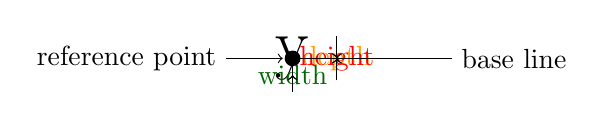
\begin{tikzpicture}
    \inClass{\uncover<1>}{\node at (0.5\wb, 0) {\raisebox{\hb}{\fontsize{120}{126}\selectfont y}};}
     \inClass{\uncover<2,3>}{\node at (0.5\wb, 0) {\raisebox{\hb}{\boxingDimF}};}
     \inClass{\uncover<3>}{\fill(0,0) circle (0.1cm);
     \node(rp) at (0,0) {};
     \node(rpt) at (-6em, 0) {reference point};
     \draw[->] (rpt) -- (rp);
     \node(bl) at (\wb+8em, 0) {base line};
     \draw (\wb,0) -- (bl);
     
     \node(wdth) at (0.5\wb, -\db-1.4ex) {\color{green!40!black}width};
     \draw[<-] (0, -\db-1.4ex) -- (wdth);
     \draw[->] (wdth) -- (\wb, -\db-1.4ex);
     \draw (0, -\db) -- +(0, -2.8ex);
     \draw (\wb, -\db) -- +(0, -2.8ex);
     
     \node(dpth) at (\wb+1.6em, -0.5\db) {\color{red!40!yellow}depth};
     \draw[<-] (\wb+1.6em, 0) -- (dpth.north);
     \draw[->] (dpth.south) -- (\wb+1.6em, -\db);
     \draw (\wb, -\db) -- +(3.2em, 0);

     \node(hght) at (\wb+1.6em, +0.5\hb) {\color{red}height};
     \draw[<-] (\wb+1.6em, 0) -- (hght.south);
     \draw[->] (hght.north) -- (\wb+1.6em, \hb);
     \draw (\wb, \hb) -- +(3.2em, 0);}
\end{tikzpicture}
     
     \skfootnote{\stExC{https://tex.stackexchange.com/questions/40977/confused-with-tex-terminology-height-depth-width}}
\end{frame}

\begin{frame}
     
\newcommand{\boxingDim}[1]{{%
\ifcsname boxtodimen\endcsname%
\else%
\newbox\boxtodimen%
\newdimen\hb%
\newdimen\db%
\newdimen\wb%
\fi%
\leavevmode 
\setbox\boxtodimen=\hbox{#1}%
\hb=\the\ht\boxtodimen%
\db=\the\dp\boxtodimen%
\wb=\the\wd\boxtodimen%
\hbox to \wb{%
    \hbox to 0pt{\box\boxtodimen}%
    \hbox to 0pt{\vbox to 0pt{\hbox{%
        \leavevmode 
        \hbox to 0pt{\raisebox{0pt}[0pt][0pt]{\color{green!40!black}\rule{\wb}{1.7pt}}}%width
        \hbox to 0pt{\raisebox{0pt}[0pt][0pt]{\rule{\wb}{0.4pt}}}%width2
        \hbox to 0pt{\raisebox{0pt}[0pt][0pt]{\color{red}\rule{1.7pt}{\hb}}}%height
        \hbox to 0pt{\raisebox{-\db}[0pt][0pt]{\color{red!40!yellow}\rule{1.7pt}{\db}}}%depth
    }}}%
    \hbox to 0pt{\vbox to 0pt{\hbox{%
        \hbox to 0pt{\raisebox{-\db}[0pt][0pt]{\rule{0.4pt}{\dimexpr\hb+\db}}}%left
        \hbox to 0pt{\hbox to \wb{}\raisebox{-\db}[0pt][0pt]{\rule{0.4pt}{\dimexpr\hb+\db}}}%right
        \hbox to 0pt{\raisebox{\hb}[0pt][0pt]{\rule{\wb}{0.4pt}}}%top
        \hbox to 0pt{\raisebox{-\db}[0pt][0pt]{\rule{\wb}{0.4pt}}}%bottom
    }}}%
}%
}%
}

\centering
% \boxingDim{
\only<1,2,3>{\leavevmode\hbox{\fontsize{120}{126}\selectfont\boxingDim{{g}}\incPause\boxingDim{f}\incPause\boxingDim{\textit{y}}\boxingDim{\textit{:}}\boxingDim{.}}}
% }
\only<4>{\boxingDim{{\fontsize{120}{126}\selectfont\boxingDim{{g}}\incPause\boxingDim{f}\incPause\boxingDim{\textit{y}}\boxingDim{\textit{:}}\boxingDim{.}}}}

\end{frame}

\inclassFrame{
\begin{frame}{Try it out!}\relax

Download and upload \texttt{boxplay.sty} and look at the ``sizes'' of different letters or worlds using \ccol\boxingDim:

\lstinputlisting[linerange={1-7, 14-15}]{boxplay.tex}

\end{frame}
}

\begin{frame}\relax
\centering\Huge \TeX\ boxes
\end{frame}

\begin{frame}[t]{``Horizontal'' boxes}{\TeX-way}\relax

    \posesPicturesOverlay{hboxmy}{
            {38-38}{\ccol{\hbox} create box around the text. The box will never split in linebreak.}, 
            {38-40}{You can specify the length of the box with keyword \ccol{to}},
            {38-41}{You even can set the box to negative size},
            {38-41,44-45}{Another keyword, \ccol{spread} is the addition width},
            {38-41,44-47}{also both positive and negative}
            }

\skfootnote{\tugC{https://www.tug.org/utilities/plain/cseq.html\#hbox-rp}}

\end{frame}

\begin{frame}[fragile]{``Horizontal'' boxes}{Usage}\relax
    \begin{columns}
    \begin{column}{0.4\textwidth}
     \verb|\hbox to -1pt{/}=|    
    \end{column}
    \begin{column}{0.4\textwidth}
         \hbox{\hbox to -1pt{/}=}
    \end{column}
    \end{columns}
    
    \begin{columns}
    \begin{column}{0.4\textwidth}
    \small
    \begin{verbatim}
\begin{tabbing}
\hbox to 4em{}\=\hbox to 4em{}\kill
a \> b\\
hello\> world!
\end{tabbing}
    \end{verbatim}     
    \end{column}
    \begin{column}{0.4\textwidth}
     \begin{tabbing}
          \hbox to 4em{}\=\hbox to 4em{}\kill
          a \> b\\
          hello\> world!
     \end{tabbing}
         
    \end{column}
    \end{columns}
     
\end{frame}

\begin{frame}[t]{``Vertical'' boxes}{\TeX-way}\relax
    \posesPicturesOverlay{vboxmy}{
            {46-47}{\ccol{\vbox} create box around the text}, 
            {46-49}{You can specify the height of the box with keyword \ccol{to}},
            {46-49,52-55}{You even can set the box to negative size, use \ccol{spread}. But depth will remain the same},
            {46-49,52-55,58-59}{There is another box, \ccol\vtop},
            {46-49,52-55,58-61}{it will change the depth for you}
            }

\skfootnote{\tugC{https://www.tug.org/utilities/plain/cseq.html\#vbox-rp}, \tugC{https://www.tug.org/utilities/plain/cseq.html\#vtop-rp}}
\end{frame}

\begin{frame}[t]{Move boxes\magicPage}\relax
\posesPicturesOverlay{moveboxmy}{
    {39-39}{\ccol\raise\ and \ccol\lower\ for horizontal boxes}, 
    {39-39,41-46}{\ccol\moveleft\ and \ccol\moveright\ for vertical boxes}
}
     \skfootnote{\tugC{https://www.tug.org/utilities/plain/cseq.html\#raise-rp} \tugC{https://www.tug.org/utilities/plain/cseq.html\#lower-rp} \tugC{https://www.tug.org/utilities/plain/cseq.html\#moveleft-rp} \tugC{https://www.tug.org/utilities/plain/cseq.html\#moveright-rp}}
\end{frame}

\begin{frame}\relax
\centering\Huge \LaTeX\ boxes
\end{frame}

\begin{frame}[t]{Horizontal boxes}\relax
\posesPicturesOverlay{mboxmy}{
    {39-40}{\ccol\mbox\ and \ccol\makebox\ are like \ccol\hbox}, 
    {39-41}{\ccol\makebox\ has a width as an optional param},
    {39-41,43-46}{... and \ccol\makebox\ has text location as second optional param}
}
     \skfootnote{\lmanc{20.1}[179] \wikiC{https://en.wikibooks.org/wiki/LaTeX/Boxes\#makebox_and_mbox}}
\end{frame}

\inClass{
\begin{frame}[t]{Paragraph boxes}\relax
\twocolImg{
\lstinputlisting[linerange={1-10}]{parboxmyInc.tex}
}{parboxmyInc}

% \ccol\parbox\ give you a box of text with some width and center vertical position.

\inclassFrag{Add a \texttt{boxplay.sty} and wrap the \ccol\parbox\ with \ccol\boxingDim\string\parbox\{\...\}\{...\} or \ccol\boxingDimHug\string\parbox\{\...\}\{...\}}[-1]
\end{frame}}

\begin{frame}[t]{Paragraph boxes\preMagicPage}\relax
\vspace*{-2ex}
\posesPicturesOverlay{parboxmy}{
    {44-44}{\ccol\parbox\ give you a box of text with some width. Also there are \ccol\pbox\ and \ccol{minipage} envirument}, 
    {44-44, 48-48}{It is just a box with  a big depth},
    {44-44, 48-50}{You can specify the position.\\ \ccol\parbox\ is useful when you want to put two lines to some command, that accepts only one line. Footnotes in the lectures use it.}
}
     \skfootnote{\lmanc{20.3}[181] \lmanc{8.18}{73} \wikiC{https://en.wikibooks.org/wiki/LaTeX/Boxes\#parbox,_minipage,_and_pbox}}
\end{frame}

\begin{frame}[fragile]{Boxes-modifiers\magicPage}\relax
\twocolImg{
\lstinputlisting[linerange={13-21, 25-25, 28-28}]{raiseboxmy.tex}
}{raiseboxmy}
 
 \ccol\raisebox\verb|{lift}[height][depth]{text}| change the text position. \ccol{\rotatebox} rotates the text, \ccol\scalebox\ scales it
\skfootnote{\lmanc{20.4}[182] \lmanc{22.3.2}[198] \lmanc{22.3.3}[199] \wikiC{https://en.wikibooks.org/wiki/LaTeX/Boxes\#box_modifiers}}
\end{frame}



